\chapter{Bevezetés}

\begin{figure}[b!]
	\begin{center}
		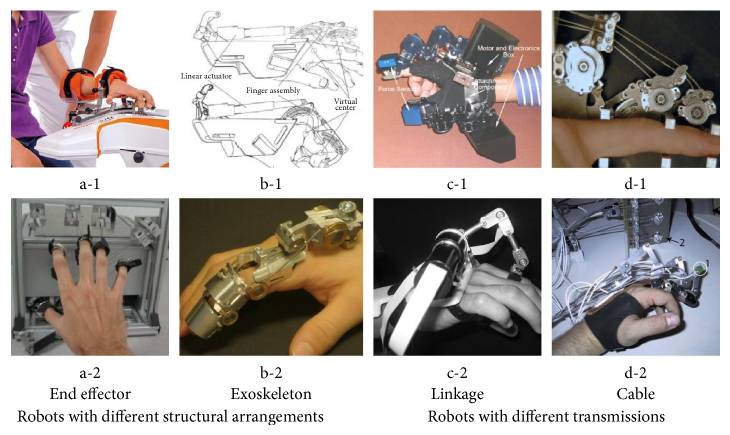
\includegraphics[width=12cm]{images/hand_rehab_robot_types.jpeg}
		\caption{A kéz rehabilitációjánál alkalmazott robotok típusai}\label{fig:hand_rehab_robot_types}
	\end{center}
\end{figure}

A sztrók évente közel 30 000~\citep{Bereczki2023} embert érint ma Magyarországon. A betegség szövődményei között gyakori 
a beszéd-, látás-, vagy mozgászavar, de akár teljes bénulást is okozhat. Az egészségügyi robotok alkalmazása a 
rehabilitáció során elősegítheti a hatékonyabb gyógyulást~\citep{Chang2013}. A kéz rehabilitációjának optimalizálása 
különösen fontos, hiszen alapvető szerepe van a mindennapi feladatok elvégzésében. A kézfej méretéből és ízületeinek számából 
adódóan sajátos kihívásokkal kell megbirkózni egy rehabilitációs robot megtervezésénél.
Az irodalomban megjelenő megoldások főbb típusai közül szemléltet párat az~\ref{fig:hand_rehab_robot_types}. ábra~\citep{Yue2017}.
Két fő kategóriát lehet megkülönböztetni a robot és a felhasználó fizikai kapcsolatát tekintve. Vannak teljesen 
különálló egységek és olyan megoldások, melyeket a felhasználó visel. Az ujjakat lehet külön-külön vagy 
csoportokban mozgatni. A meghajtás lehet elektromos, pneumatikus vagy hidraulikus, de akár piezoelektromos vagy 
alak emlékező fémötvözeten alapuló is. A elektromos meghajtás igen elterjedt, mert széles választék áll rendelkezésre különféle motorokból, 
valamint kedvező az ára és igen megbízható. Az erőátvitel lehet közvetlen, gyakran azonban közvetítő elem (csuklók, kábelek) 
segítségével történik. A páciens aktív részvétele jobb eredményeket mutat a passzív, erőkifejtés nélküli mozgatással 
szemben~\citep{Remsik2016}, ezért elengedhetetlen a páciens mozgási szándékáról valamilyen visszajelzés közvetítése a robot felé.
Ezután a robot a pácienssel összhangban hajthatja végre a gyakorlatot.
A szenzorokat tekintve vannak megoldások melyek a mozgásállapotot mérik (erő, nyomaték, elmozdulás)~\citep{Bauer2021}, de megjelennek 
bioelektromos jeleket mérő szenzorok is~\citep{Satakogiou}. 

A hardveren túl a szabályozó típusa szerint is csoportosíthatók a különböző megoldások. Vannak erőszabályozáson 
alapuló rendszerek~\citep{kovacs2003dynamics}, de leggyakoribbak a hibrid erő és 
pozíció szabályozáson alapuló egységek~\citep{Hua2019,Xie2021}, azonban vannak például fuzzy szabályozáson alapuló architektúrák is~\citep{Hu2023}.
A hibrid erő és pozíció szabályozásnak számos előnye van a tisztán pozíció vagy erő visszacsatolással 
szemben~\citep{hogan1984Impedance,hogan1985ImpedancePART1,hogan1985ImpedancePART2,hogan1985ImpedancePART3,kovacs2003dynamics,stepan2001vibrations}.
Ez a szabályozó típus kifejezetten jól alkalmazható ember-robot interakciót igénylő feladatoknál, mint amilyen 
a rehabilitáció is. A szabályozó referencia jele nem csupán 
az elérni kívánt pozíció vagy kifejtett nyomaték, hanem a mozgásállapot és a kifejtett
nyomaték közötti összefüggés. Ezt az összefüggést egy 
tömeg-rugó-csillapitás modell adja meg a továbbiakban, mely a következő alakban
írható fel: 
\begin{align}
    M_\RM e \ddot \theta + B_\RM e \dot \theta + K_\RM e (\theta - \theta_\RM r) = \tau_\RM e\,.
\end{align}
A modell három paraméterrel rendelkezik, $M_\RM e$ a rendszer előírt tehetetlensége, 
$B_\RM e$ a viszkózus csillapítása, és $K_\RM e$ a rugóállandója. 
$\theta_\RM r$ és $\tau_\RM e$ az elérni kívánt pozíció és a rendszerre ható külső nyomaték. 

\begin{figure}[t!]
	\begin{center}
		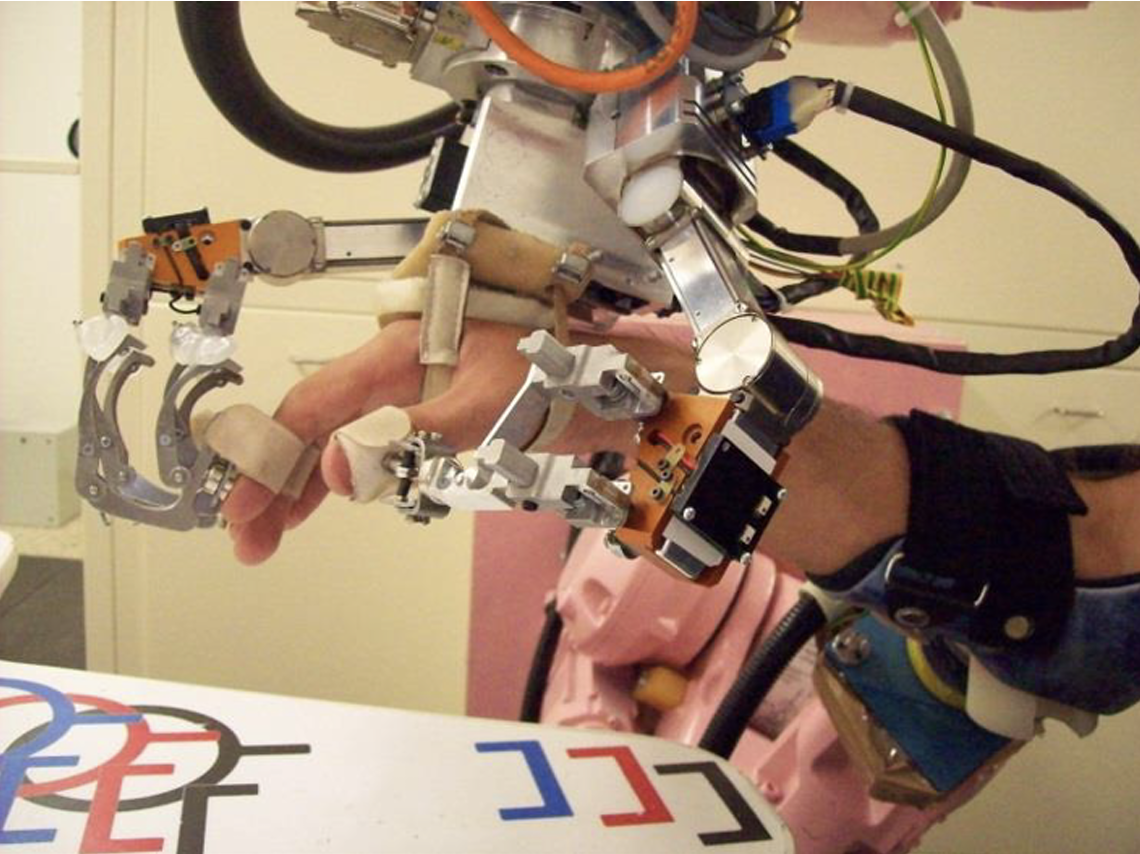
\includegraphics[width=8cm]{images/reharob_hand_module.png}
		\caption{A REHAROB rehabilitációs robot kézmodulja}\label{fig:reharob_hand_module}
	\end{center}
\end{figure}

Ez a dolgozat elsősorban az Országos Mozgásszervi Intézetben megépített REHAROB 3.0 
rehabilitációs robot kézmoduljában alkalmazott robotujj hatékonyságának javításához kíván hozzájárulni.
A robot kézmodulja az~\ref{fig:reharob_hand_module}. ábrán látható.
A REHAROB 3.0 rehabilitációs robot működhet passzív vagy aktív üzemmódban. Passzív üzemmódban előre felvett 
mozgáspályákon halad végig, míg aktív üzemmódban előre beprogramozott hétköznapi feladatok 
kivitelezésében asszisztálja a pácienst. A kézmodul közvetlen hajtással rendelkezik. A mutatóujj, a középső ujj és a
gyűrűs ujj együtt, míg a hüvelyujj külön mozgatható. A kisujj nem vesz részt a mozgatásban. Cserélhető ortézisek 
teszik lehetővé, hogy különböző kéz mérettel rendelkező páciensek is használhassák a berendezést.



A dolgozat a robotujj egyszerűsítettt egyszabadságfokú modelljére alkalmazott admittancia szabályozó stabilitását vizsgálja.
A digitális rendszerek stabilitására nagy hatással lehet az időkésés~\citep{stepan1989retarded,stepan2001vibrations}, így a 
stabilitásvizsgálat során fő szempont lesz ennek a hatásnak az elemzése.


% \begin{itemize}
%     \item Irtech: 
%     \citep{lantos2016iranyitasi1,lantos2016iranyitasi2,lantos2017iranyitasi3}
%     + MOGIS VALAMI + NEMZETKÖZI
    
%     \item Kálmán: state space, megfigyelő, stb: \citep{kalman1960new,kalman1963controllability,kalman1963mathematical,kalman1960contributions}
    
% \end{itemize}
